\section{Userstudy}

To evaluate our game we conducted a user study during the Demo Day. This allowed us to get a more or less diverse group of 12 test users, that were willing to take some of their time to fill in our questionnaire.

\subsection{Study methodology}

Our user study was done in two separate steps. Before playing the game participants filled out some classification information (age within a range and their gender) as well as information about previous knowledge on a scale from 1 to 5. We asked about familiarity with:

\begin{itemize}
	\item 3D Movies
	\item Videogames (PC)
	\item Videogames (Mobile)
	\item Augmented Reality (AR)
	\item Virtual Reality (VR)
	\item Mixed Reality (XR)
	\item Celts
	\item Celtic Runes
	\item TowerDefense Games
\end{itemize}

After playing the game we asked players if they liked the game and how much they thought they learned about runes on a 1 to 5 scale. Finally we let them fill out a six-question test to see how much they remembered about runes after playing the first few levels.
The test consisted of remembering the name of three different runes and drawing three other runes based on their name.
It's important to note that participants did not know they will be tested after playing the game, so they did play for fun not for knowledge.
Unfortunately, but understandably in the Demo Day environment, not all players had the time to play long enough to unlock two runes asked for in the end of the test, so our results are a little bit flawed in that regard and learning success might actually be better.
Lastly, the participants had the option to suggestion for improvement in a free-text field at the end of the questionnaire.

\subsection{Study evaluation}

The majority of participants were very familiar with AR/VR which is most likely due to us handing out the questionnaire during Demo Day, the most relevant event for games engineering students.
On a scale from 1 (bad) to 5 (good), previous knowledge about Celts was self-rated at ~1.92. After playing the game the self-rating on how much the test users learned about the Celtic culture was at 2.5.
The test group was able to score 3.3 out of 6 possible points in the drawing quiz part.
Overall, most of the testers liked the general tower defense concept with a score of 3.9 and liked our game with a score of 4.1. So the Celtic aspect increased the fun the testers had while playing the game.

\begin{figure}[ht]
	\centering
	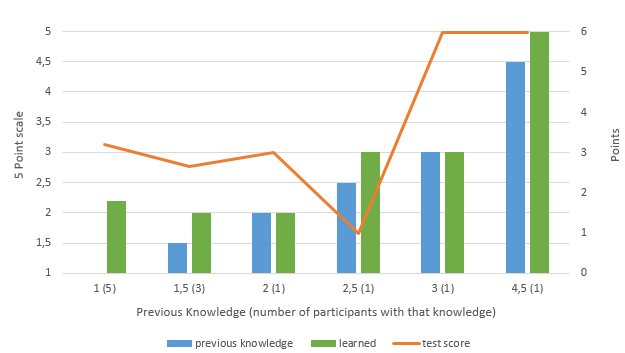
\includegraphics[width=0.95\linewidth]{figures/knowledge-learned.png}
	\caption{How much did participants learn based on previous knowledge.}
	\label{fig:knowledge-learned}
\end{figure}


Figure~\ref{fig:knowledge-learned} illustrates how much participants learned based on their previous knowledge. We see that for the majority of knowledge groups there was an increase in perceived knowledge after playing the game. No participant knew less about Celtic runes than before playing the game. Figure~\ref{fig:knowledge-learned} also shows a positive correlation between the perceived learning success and the test score of participants.
Although it must be noted here, that we need a higher number of participants ideally from a more diverse group to draw sound conclusions. The raw test results can be found in Appendix~\ref{appendix-userstudy}.

From the free-text suggestions, the most asked for improvement was to reduce the amount of unlocked runes for every level in the campaign mode. For Demo Day we did not create a fully fleshed out campaign. We tried to keep the campaign relatively short to make it playable in a shorter amount of time, to make the game not as time consuming as it would be in the final version, but this was partly overwhelming for our players.
Furthermore, the marker-tracking performance was an issue for some testers despite our efforts to make it as stable as possible. Possible ways of improving AR further would be using a better device (computing power and better camera) and/or using advanced AR-libraries (ARCore/ARKit).

